% Type of the document
\documentclass{beamer}

% elementary packages:
\usepackage{graphicx}
\usepackage[latin1]{inputenc}
\usepackage[T1]{fontenc}
\usepackage[english]{babel}
\usepackage{listings}
\usepackage{xcolor}
\usepackage{eso-pic}
\usepackage{mathrsfs}
\usepackage{url}
\usepackage{amssymb}
\usepackage{amsmath}
\usepackage{multirow}
\usepackage{hyperref}
\usepackage{booktabs}

% additional packages
\usepackage{bbm}

% packages supplied with ise-beamer:
\usepackage{cooltooltips}
\usepackage{colordef}
\usepackage{beamerdefs}
\usepackage{lvblisting}

% Change the pictures here:
% logobig and logosmall are the internal names for the pictures: do not modify them. 
% Pictures must be supplied as JPEG, PNG or, to be preferred, PDF
\pgfdeclareimage[height=2cm]{logobig}{hulogo}
% Supply the correct logo for your class and change the file name to "logo". The logo will appear in the lower
% right corner:
\pgfdeclareimage[height=0.7cm]{logosmall}{Figures/LOB_Logo}

% Title page outline:
% use this number to modify the scaling of the headline on title page
\renewcommand{\titlescale}{1.0}
% the title page has two columns, the following two values determine the percentage each one should get
\renewcommand{\titlescale}{1.0}
\renewcommand{\leftcol}{0.6}

% Define the title.Don't forget to insert an abbreviation instead 
% of "title for footer". It will appear in the lower left corner:
\title[Quiz 1]{Selected topics in Mathematical Statistics, Quiz 1}
% Define the authors:
\authora{Malte Esders} % a-c
\authorb{}
\authorc{}

% Define any internet addresses, if you want to display them on the title page:
\def\linka{http://lvb.wiwi.hu-berlin.de}
\def\linkb{}
\def\linkc{}
% Define the institute:
\institute{Humboldt--Universit�t zu Berlin \\}

% Comment the following command, if you don't want, that the pdf file starts in full screen mode:
%\hypersetup{pdfpagemode=FullScreen}

%Start of the document
\begin{document}

% create the title slide, layout controlled in beamerdefs.sty and the foregoing specifications
\frame[plain]{
\titlepage
}

%%%%%%%%%%%%%%%%%%%%%%%%%%%%%%%%%%%%%%%%%%%%%%%%%%%%%%%%%%%%%%%%%%%%%%%%%%%%%%%%%%%%%%%%%%%%%%%%%%%%%%%%%%%%%%%%%%%%%%%%
\section{Problem Description}

\frame{
\frametitle{Problem Description}
Quiz 1: Relate Interquartile Range (IQR) to Standard Deviation (SD) under some distributions.
}


%%%%%%%%%%%%%%%%%%%%%%%%%%%%%%%%%%%%%%%%%%%%%%%%%%%%%%%%%%%%%%%%%%%%%%%%%%%%%%%%%%%%%%%%%%%%%%%%%%%%%%%%%%%%%%%%%%%%%%%%
\section{Uniform Distribution}

\frame{
\frametitle{Uniform Distribution}
Probability density function:
\begin{align} 
\begin{split}
	f_X(x) = \frac{1}{b-a}
\end{split}					
\end{align}

Cumulative density function:
\begin{align} 
\begin{split}
	F_X(x) = \frac{x-a}{b-a}
\end{split}					
\end{align}

Quantile function:
\begin{equation}
\begin{aligned} 
	F_X^{-1}(p) = a + p(b-a)  \\
\end{aligned}
\end{equation}
}

\frame{
The quantiles:
\begin{equation}
\begin{aligned} 
	\xi_{\frac{1}{4}} = F^{-1}(\tfrac{1}{4}) = a + \frac{1}{4}(b-a) \\
	\xi_{\frac{3}{4}} = F^{-1}(\tfrac{3}{4}) = a + \frac{3}{4}(b-a)
\end{aligned}
\end{equation}

So, the Interquartile Range is
\begin{equation}
	IQR = \frac{1}{2}(b-a)
\end{equation}
}

\frame{
And the Standard Deviation of the uniform distribution is known to be
\begin{equation}
	\text{SD} = \frac{(b-a)}{\sqrt{12}}
\end{equation}

so the ratio of IQR to SD is

\begin{equation}
	\frac{IQR}{SD} = \frac{\frac{1}{2}}{\frac{1}{\sqrt{12}}} = \sqrt{3}
\end{equation}
}

%%%%%%%%%%%%%%%%%%%%%%%%%%%%%%%%%%%%%%%%%%%%%%%%%%%%%%%%%%%%%%%%%%%%%%%%%%%%%%%%%%%%%%%%%%%%%%%%%%%%%%%%%%%%%%%%%%%%%%%%
\section{Exponential Distribution}
\frame{
\frametitle{Exponential Distribution}

Probability density function:
\begin{align} 
\begin{split}
	f_X(x) = \lambda e^{-\lambda x}
\end{split}					
\end{align}

Cumulative density function:
\begin{align} 
\begin{split}
	F_X(x) = 1-e^{-\lambda x}
\end{split}					
\end{align}
}

\frame{
Deriving the quantile function:
\begin{equation}
\begin{aligned} 
	F_X^{-1}(p) &= x_p  \\
	F_X(x_p) = p &= 1-e^{-\lambda x_p} \\
	e^{-\lambda x_p} &= 1-p \\
	x_p &= -\frac{\ln(1-p)}{\lambda} \\
\end{aligned}
\end{equation}

So, $F_X^{-1}(p)$ is: 
\begin{align} 
\begin{split}
	F_X^{-1}(p) = -\frac{\ln(1-p)}{\lambda}
\end{split}					
\end{align}
}

\frame{
Quantiles:
\begin{equation}
\begin{aligned} 
	\xi_{\frac{1}{4}} = F^{-1}(\tfrac{1}{4}) = -\frac{\ln(1-\frac{1}{4})}{\lambda} = \frac{\ln{\frac{4}{3}}}{\lambda}\\
	\xi_{\frac{3}{4}} = F^{-1}(\tfrac{3}{4}) = -\frac{\ln(1-\frac{3}{4})}{\lambda} = \frac{\ln{4}}{\lambda}
\end{aligned}
\end{equation}

So, the Interquartile Range is
\begin{equation}
	IQR = \frac{\ln{4} - \ln{\frac{4}{3}}}{\lambda} = \frac{\ln{3}}{\lambda}
\end{equation}
}

\frame{

The Standard Deviation of the exponential distribution is known to be $\frac{1}{\lambda}$, so the ratio of IQR to SD is

\begin{equation}
	\frac{IQR}{SD} = \lambda \ln{3} \approx \lambda * 1.098
\end{equation}
}


\section{Normal Distribution}
%%%%%%%%%%%%%%%%%%%%%%%%%%%%%%%%%%%%%%%%%%%%%%%%%%%%%%%%%%%%%%%%%%%%%%%%%%%%

\frame{
\frametitle{Normal Distribution}
For the Normal Distribution, the cumulative and quantile distributions can't be expressed in elementary functions, therefore one has to use numerical approximations.\\
The first and third quantiles of the standard normal distribution are

\begin{equation}
\begin{aligned} 
	\xi_{\frac{1}{4}} = \Phi^{-1}(\tfrac{1}{4}) &= -0.68 \\
	\xi_{\frac{3}{4}} = \Phi^{-1}(\tfrac{3}{4}) &= 0.68
\end{aligned}
\end{equation}
\\
}
\frame{
So the interquartile range is $IQR = 0.68-(-0.68) = 1.36$. Since the standard deviation of the standard normal distribution is 1, the ratio is

\begin{equation}
	\frac{IQR}{SD} = \frac{1.36}{1} = 1.36
\end{equation}
}




% Define the end of the document:

\section{Visual illustration}
\frame{
\begin{figure}[ht]
	\begin{center}
		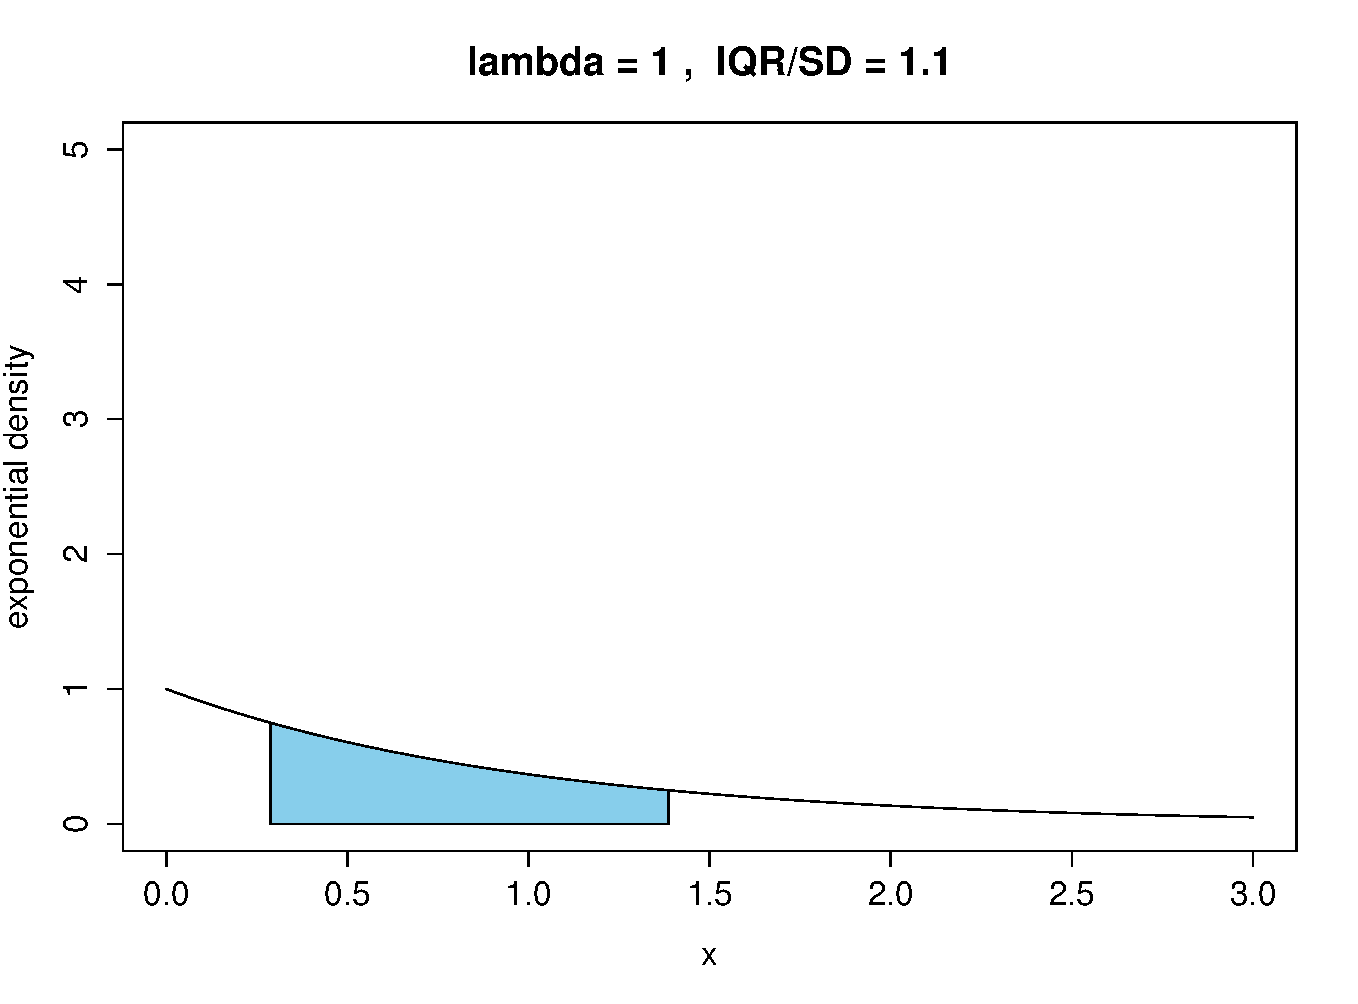
\includegraphics[width=0.5\textwidth, height = 5.0cm]{exp_plot_1}
		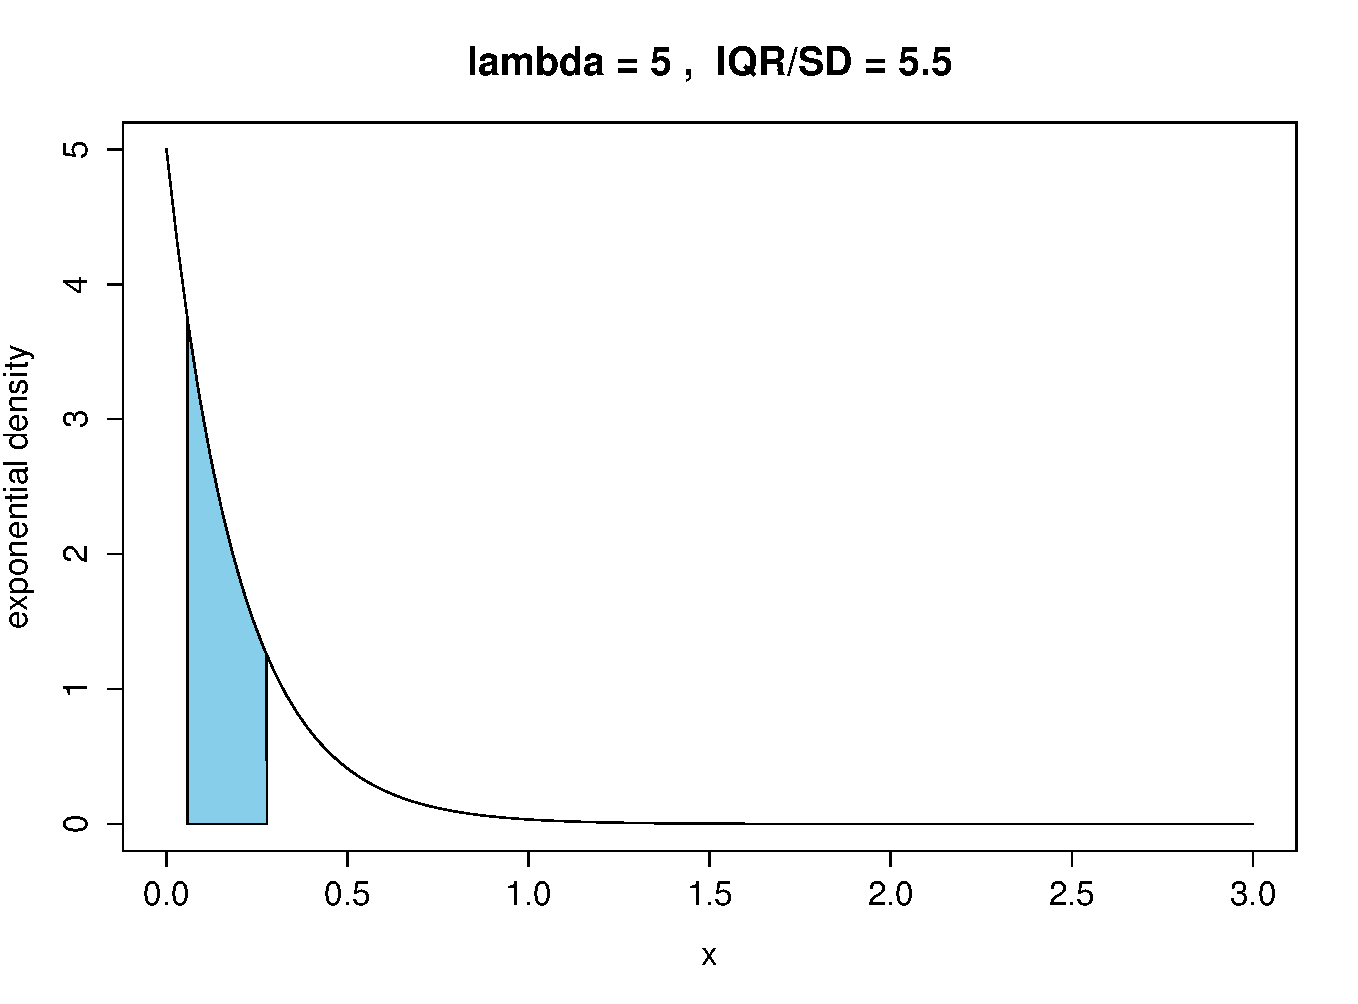
\includegraphics[width=0.5\textwidth, height = 5.0cm]{exp_plot_2}
		\caption{Exponential Distribution for different values of lambda, colored region is interquartile range}\label{fig:exp}
	\end{center}
\end{figure}
}
\end{document}
